\section{Methods}
Given the different methods that can be used for training a reinforcement learning agent an environment has been set up where one can easily change the type of opponents within the pommerman environment. Furthermore the ability to change between a value-function-based method such as Q-learning, and a policy search method realised with the gradient estimator REINFORCE has been implemented.\cite{sutton1998a} To make the starting point more simple it is made possible to hold the board static, rather than using an new randomly generated board every time as is the case in figure \ref{fig:pomIntro}. The structure of the environment can be seen in figure \ref{fig:uml}.

\begin{figure}[htb]
    \centerline{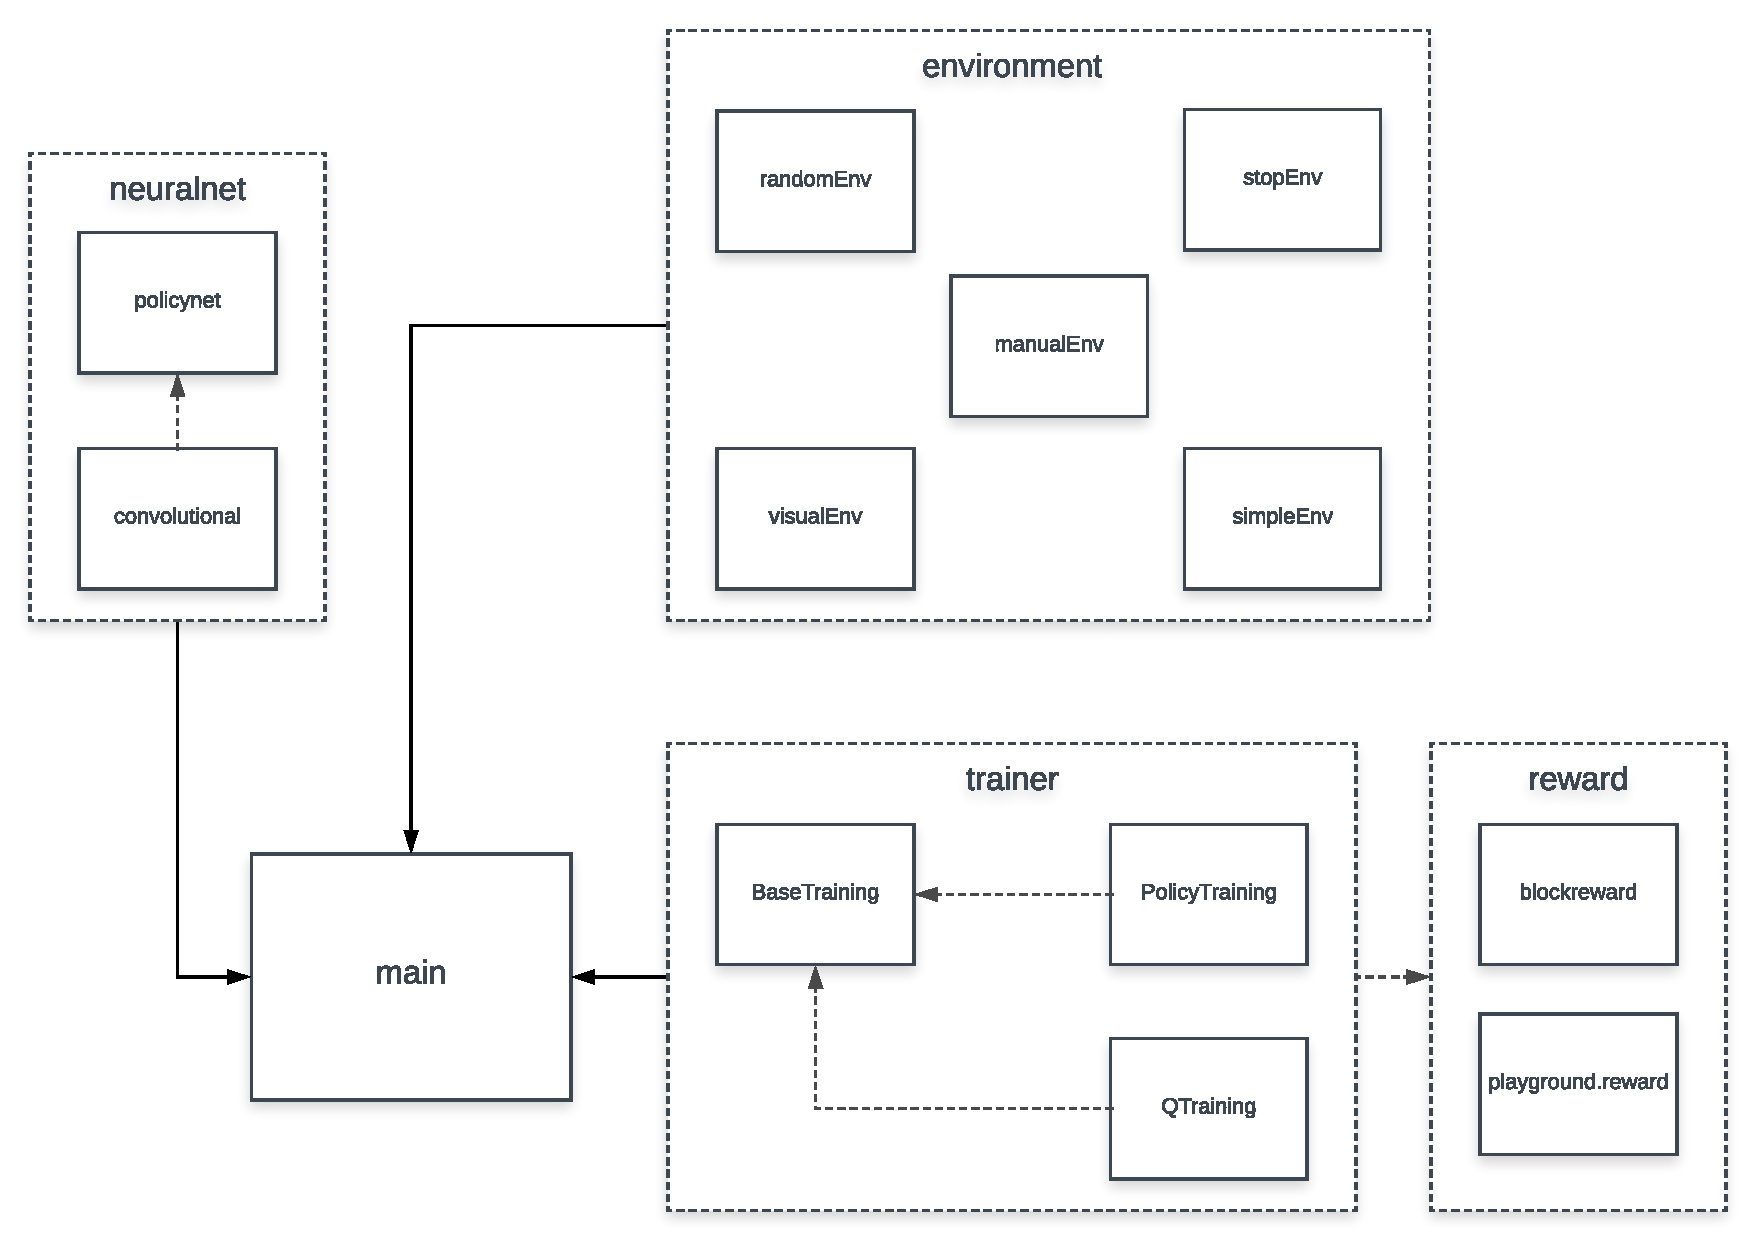
\includegraphics[width=0.8\linewidth]{docs/article/inputs/02456-UML.pdf}}
    \caption{UML of workflow.}\label{fig:uml}
\end{figure}



% Methods used in our solution, could here be network choice, algorithm, parameter-choice etc.
% REINFORCE paper reference
% Network?
% Why was the chosen methods used

% http://incompleteideas.net/book/bookdraft2017nov5.pdf
\subsection{Reinforcement Learning: An Introduction} % Monte carlo, n-step TD, REINFORCE, actor critic.

% Questions to answer:
% - Why was the method used?
% - How does it work?

\subsection{Reinforce algorithm}

\subsection{Deep Q-learning}
% mention bomberman article

\subsection{Feature engineering}

\subsection{Convolutional network}

\subsection{Exploration / Exploitation (episilon decay)}
\begin{figure}[htb]
    \centerline{\includegraphics[width=0.8\linewidth]{}}
    \caption{UML of workflow.}\label{fig:uml}
\end{figure}
\begin{figure}[htb]
    \centerline{\includegraphics[width=0.8\linewidth]{}}
    \caption{UML of workflow.}\label{fig:uml}
\end{figure}

\subsection{Static board}
% Static board to reduce complexity

\subsection{Reward function}
% Simple +/-1 1
% Cite bomberman/our tweaked version
Functionality to change the reward function has also been introduced. Besides the standard reward function that comes with the pommerman environment, where the agents receives a score of 1 for winning and -1 for loosing, some agents were trained with reward shaping. The general motivation for introducing the reward shaping was in an attempt to encourage the agent to avoid getting stuck in a local minimum. One of the reward functions used for this was the same as was used by \cite{kormelink2018exploration} and can be seen in table~\ref{tab:rew}. This reward function was introduced to encourage the agent to explore the map by rewarding the agent for blowing up wall and giving it negative reward for moving and performing illegal actions, like walking into a wall. I.e. if the agent wish to receive a total positive rewards it has to blow up opponents or walls.

\begin{table}[htb]
    \centerline{
        \begin{tabular}{|l|r|}
            \hline
            action                  & reward   \\ 
            \hline
            Blow up opponent 		& $100$	\\
            Blow up wall  			& $30$  \\
            Perform action			& $-1$	\\
            Perform illegal action	& $-2$	\\
            Die  					& $-300$\\
            \hline
        \end{tabular}
    }
    \caption{A table with an example of reward shaping.}\label{tab:rew}
\end{table}